\documentclass[a4paper]{report}
\usepackage{listings}
\usepackage{enumitem}
\usepackage{mdframed}
\usepackage{graphicx} % Required for the inclusion of images

\title{CEEN 8886: Homework 6}
\date{2017-04-19}
\author{Kelly Boswell}

\makeatletter
\DeclareRobustCommand{\textsupsub}[2]{{%
  \m@th\ensuremath{%
    ^{\mbox{\fontsize\sf@size\z@#1}}%
    _{\mbox{\fontsize\sf@size\z@#2}}%
  }%
}}
\makeatother

\begin{document}

\maketitle

\pagenumbering{gobble}

\newpage

\pagenumbering{arabic}

% Problem 1
\section{Problem 1 --- 3G (UMTS) Security}

\subsection{Discuss the new infrastructure requirements in moving from a GSM
            network to UMTS.}

In GSM, the main architectural components are illustrated in Figure \ref{fig:prob1a}.
They are the Mobile Station (MS) which includes the subscriber's SIM card;
the Base Station Subsystem which consists of Base Station
Controller (BSC) and the Base Transceiver Station (BSS); and the Network Subsystem
which consists of the Home Location Register (HLR), the Visitor Location Register
(HLR), the Equipment Identity Register (EIR), the Authentication Centre (AuC), and
the Mobile Service Switching Center (MSC).

In UMTS, the main architectural components are illustrated in Figure \ref{fig:prob1b}
and Figure \ref{fig:prob1c}.  They are the User Equipment (UE) which includes the
users USIM card; the UMTS Terrestrial Radio Access Network (UTRAN) which is composed
of Node Bs used to connect the UE to a the core network via a Radio Network Controller
(RNC); and the core network which consists of the HLR, VLR, EIR, MSC, and AuC but includes
new components to support General Packet Radio Service (GPRS) --- intruduced in 2.5G --- 
for packet-based wireless communications to support TCP/IP communication protocols. These
new components are the Serving GPRS Support Node (SGSN) and the Gateway GPRS Support Node
(GGSN). The core network also consists of a Gateway Mobile Switching Centre (GMSC) used to
interface to external networks.

\begin{figure}
\begin{mdframed}
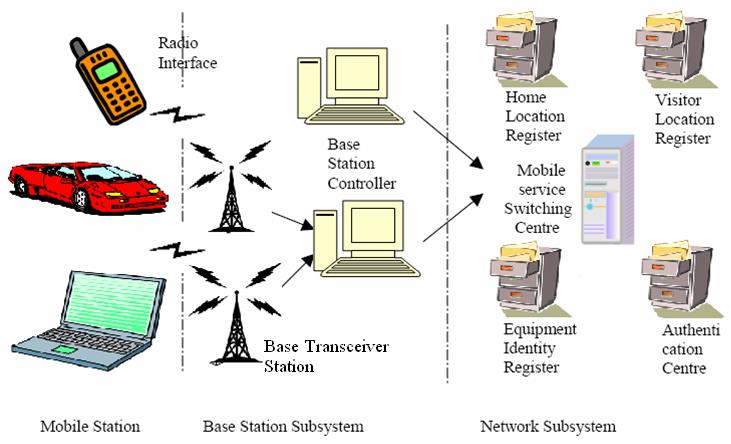
\includegraphics[scale=0.4]{GSM_Architecture.png}
\caption{GSM Architecture}
\label{fig:prob1a}
\end{mdframed}
\end{figure}

\begin{figure}
\begin{mdframed}
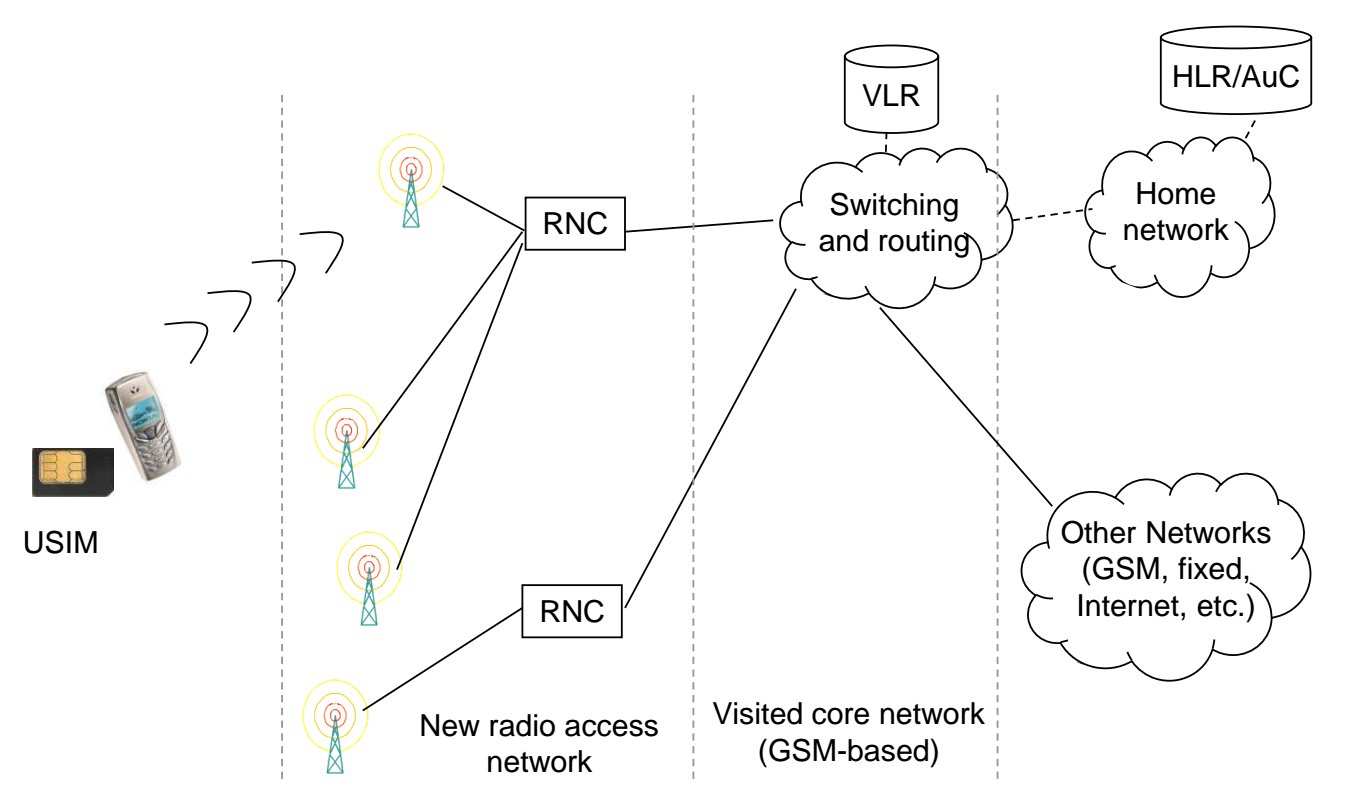
\includegraphics[scale=0.2]{UMTS_Architecture1.jpg}
\caption{3GPP Architecture --- UMTS}
\label{fig:prob1b}
\end{mdframed}
\end{figure}

\begin{figure}
\begin{mdframed}
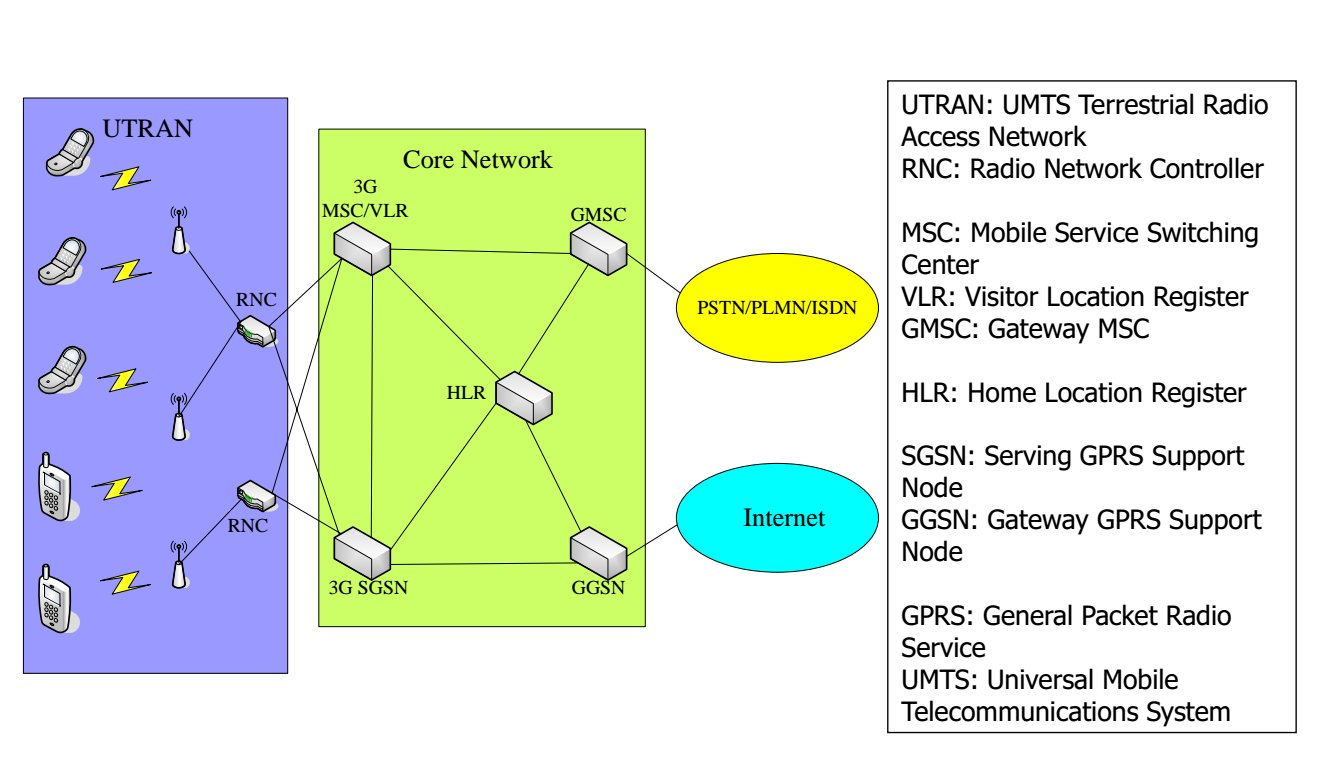
\includegraphics[scale=0.2]{UMTS_Architecture2.jpg}
\caption{3GPP Architecture --- UMTS}
\label{fig:prob1b}
\end{mdframed}
\end{figure}

%Problem 2
\section{Problem 2 --- LTE Security}

\subsection{Illustrate the improvements of LTE security over UMTS security.
            Give detailed explanations.}

\begin{enumerate}
\item Network Access Security
    \begin{enumerate}
    \item Serving network identity (SN ID) has been added to the EPS AKA procedure to avoid attacks 
             such as redirection attacks and false base station attacks.
    \item On top of the security functions at the access stratum (AS) level between the User Equipment
             (UE) and the eNB, new security functions at the non access stratum (NAS) level between the 
             UE and the Mobility Management Entity (MME) have been included.
    \item The new root key K\textsubscript{ASME}, computed by the Home Server Subscriber (HSS), will be delivered
             to the Mobility Management Entity (MME) or the serving network (SN).
    \item The key set identifier KSI\textsubscript{ASME} is embedded in the user authentication request message
             transmitted to the UE by the MME.
    \item A new key heirarchy is introduced to protect the security of the signaling and user data traffic.
    \end{enumerate}
\item Security in Handover Processes
    \begin{enumerate}
    \item Intra E-UTRAN mobility: The current eNB and the target eNB are managed by the same MME
        \begin{enumerate}
        \item A new key management mechanism is designed with different ways to derive the new eNB keys
                 based on vertical or horizontal key derivations.
        \item A MME and the UE shall derive a K\textsubscript{eNB} and a next hop (NH) parameter from the K\textsubscript{ASME},
                 which is derived by the UE and the MME after an initial access authentication.
        \item In the initial setup, K\textsubscript{eNB} is derived directly from the K\textsubscript{ASME}, and is then associated with a
                 virtual NH parameter with a NH chaining counter (NCC)  value to be zero. The UE and the eNB
                 use the K\textsubscript{eNB} to secure the communication on the air interface.
        \item In handovers, a new session key used between the UE and the target eNB, K\textsupsub{*}{eNB},
                 is derived from either the active K\textsubscript{eNB} or from the NH parameter.
        \end{enumerate}
    \item Mobility between the E-UTRAN and UTRAN/GERAN
        \begin{enumerate}
        \item For the handover from the E-UTRAN to the UMTS Terrestrial Radio Access Network (UTRAN) or the
                 GSM EDGE Radio Access Network (GERAN):
            \begin{enumerate}
            \item the UE and the MME shall first derive a CK and IK from the K\textsubscript{ASME}
            \item upon receiving CK' || IK' with KSI' from the MME, the target Service GPRS Supporting Node (SGSN) and
                     the UE shall replace all stored parameters CK, IK, KSI, with CK', IK', and KSI'.
            \item the UE and the target SGSN shall use CK' and IK' to derive the General Packet Radio Service (GPRS)
                     K\textsubscript{c}.
            \end{enumerate}
        \item For the handover from the UTRAN/GERAN to the E-UTRAN:
            \begin{enumerate}
            \item The target MME shall derive K\textsupsub{'}{ASME} from CK and IK or GPRS K\textsubscript{c} received
                     from the SGSN.
            \item The UE shall also execute the above same procedure as the MME to derive K\textsupsub{'}{ASME}.
            \item The target MME and the UE shall derive K\textsubscript{eNB} and the corresponding NAS keys according
                     to the key heirarchy of LTE. 
            \end{enumerate}
        \end{enumerate}
    \item Mobility between E-UTRAN and non-3GPP access networks
        \begin{enumerate}
        \item There are several different mobility scenarios between heterogeneous access systems in the LTE networks:
            \begin{enumerate}
            \item Handovers from trusted or untrusted non-3GPP access networks to the E-UTRAN
            \item Handovers from the E-UTRAN to trusted or untrusted non-3GPP access networks
            \end{enumerate}
        \item The UE, the target access network and the EPC will implement a full access authentication procedure before
                 the UE handovers to the new access network.
        \item Different access authentication procedures will be executed in distinct mobility scenarios.
        \end{enumerate}
    \end{enumerate}
\end{enumerate}

%Problem 3
\section{Problem 3 --- IEEE 802.15 for WPAN Security}

Alice is using GSM cellular network to communicate with her friends.

\subsection{What is the hopping rate in Bluetooth and how many bits are
            transmitted in one slot transmission?}


\subsection{Which 802.11 LAN standards will Bluetooth interfere with?}


\subsection{What is the reason for a lower speed/lower power WPAN standard
            such as IEEE 802.15.4?}

\end{document}
